%Version 3 October 2023
% See section 11 of the User Manual for version history
%
%%%%%%%%%%%%%%%%%%%%%%%%%%%%%%%%%%%%%%%%%%%%%%%%%%%%%%%%%%%%%%%%%%%%%%
%%                                                                 %%
%% Please do not use \input{...} to include other tex files.       %%
%% Submit your LaTeX manuscript as one .tex document.              %%
%%                                                                 %%
%% All additional figures and files should be attached             %%
%% separately and not embedded in the \TeX\ document itself.       %%
%%                                                                 %%
%%%%%%%%%%%%%%%%%%%%%%%%%%%%%%%%%%%%%%%%%%%%%%%%%%%%%%%%%%%%%%%%%%%%%

%%\documentclass[referee,sn-basic]{sn-jnl}% referee option is meant for double line spacing

%%=======================================================%%
%% to print line numbers in the margin use lineno option %%
%%=======================================================%%

%%\documentclass[lineno,sn-basic]{sn-jnl}% Basic Springer Nature Reference Style/Chemistry Reference Style

%%======================================================%%
%% to compile with pdflatex/xelatex use pdflatex option %%
%%======================================================%%

%%\documentclass[pdflatex,sn-basic]{sn-jnl}% Basic Springer Nature Reference Style/Chemistry Reference Style


%%Note: the following reference styles support Namedate and Numbered referencing. By default the style follows the most common style. To switch between the options you can add or remove “Numbered” in the optional parenthesis. 
%%The option is available for: sn-basic.bst, sn-vancouver.bst, sn-chicago.bst%  
 
%%\documentclass[sn-nature]{sn-jnl}% Style for submissions to Nature Portfolio journals
%%\documentclass[sn-basic]{sn-jnl}% Basic Springer Nature Reference Style/Chemistry Reference Style

\RequirePackage{amsthm}
\documentclass[sn-mathphys-num]{sn-jnl}% Math and Physical Sciences Numbered Reference Style 
%%\documentclass[sn-mathphys-ay]{sn-jnl}% Math and Physical Sciences Author Year Reference Style
%%\documentclass[sn-aps]{sn-jnl}% American Physical Society (APS) Reference Style
%%\documentclass[sn-vancouver,Numbered]{sn-jnl}% Vancouver Reference Style
%%\documentclass[sn-apa]{sn-jnl}% APA Reference Style 
%%\documentclass[sn-chicago]{sn-jnl}% Chicago-based Humanities Reference Style

%%%% Standard Packages
%%<additional latex packages if required can be included here>

\usepackage{graphicx}%
\usepackage{multirow, hhline}%
\usepackage{amsmath,amssymb,amsfonts}%
\usepackage{mathrsfs}%
\usepackage[title]{appendix}%
\usepackage{xcolor}%
\usepackage{textcomp}%
\usepackage{manyfoot}%
\usepackage{booktabs}%
\usepackage{algorithm}%
% \usepackage{algorithmic}
\usepackage{algorithmicx}%
\usepackage{algpseudocode}%
\usepackage{listings}%
\usepackage{lmodern}
\usepackage{hyperref}

%%%%
\usepackage[markup=default]{changes}
\definechangesauthor[name={Author}, color=orange]{A}
\definechangesauthor[name={Table}, color=blue]{B}
\definechangesauthor[name={Revision}, color=purple]{C}
\usepackage{soul}
\usepackage[normalem]{ulem}
\usepackage{url}


% Inserted text:
% \added[id=A]{This sentence has been newly added to clarify our technical contributions.}

% Deleted text:
% \deleted[id=A]{This previous sentence has been removed because it lacked clarity.}

% Replaced text:
% \replaced[id=A]{We introduce a novel curriculum design tailored for radiological tasks}{Our method uses curriculum learning}.


%% as per the requirement new theorem styles can be included as shown below
\theoremstyle{thmstyleone}%
\newtheorem{theorem}{Theorem}%  meant for continuous numbers
%%\newtheorem{theorem}{Theorem}[section]% meant for sectionwise numbers
%% optional argument [theorem] produces theorem numbering sequence instead of independent numbers for Proposition
\newtheorem{proposition}[theorem]{Proposition}% 
%%\newtheorem{proposition}{Proposition}% to get separate numbers for theorem and proposition etc.

\theoremstyle{thmstyletwo}%
\newtheorem{example}{Example}%
\newtheorem{remark}{Remark}%

\theoremstyle{thmstylethree}%
\newtheorem{definition}{Definition}%

\raggedbottom
%%\unnumbered% uncomment this for unnumbered level heads

\begin{document}

\title{Joint Imbalance Adaptation for Radiology Report Generation}

%%=============================================================%%
%% GivenName	-> \fnm{Joergen W.}
%% Particle	-> \spfx{van der} -> surname prefix
%% FamilyName	-> \sur{Ploeg}
%% Suffix	-> \sfx{IV}
%% \author*[1,2]{\fnm{Joergen W.} \spfx{van der} \sur{Ploeg} 
%%  \sfx{IV}}\email{iauthor@gmail.com}
%%=============================================================%%

\author[1]{\fnm{Wang} \sur{Li}}
\author[1]{\fnm{Guangzeng} \sur{Han}}
\author[1]{\fnm{Yuexin} \sur{Wu}}
%\email{yuexin.wu@memphis.edu}
%ORCID https://orcid.org/0000-0003-1109-2599
\author[2]{\fnm{I-Chan} \sur{Huang}} %\email{i-chan.huang@stjude.org}
% \equalcont{These authors contributed equally to this work.}

\author*[1]{\fnm{Xiaolei} \sur{Huang}}\email{xiaolei.huang@memphis.edu}
% \equalcont{These authors contributed equally to this work.}

\affil[1]{\orgdiv{Department of Computer Science}, \orgname{University of Memphis}, \orgaddress{\city{Memphis}, \postcode{38152}, \state{TN}, \country{United States}}}

\affil[2]{\orgdiv{Department of Epidemiology and Cancer Control}, \orgname{St. Jude Children's Research Hospital}, \orgaddress{\city{Memphis}, \postcode{38105}, \state{TN}, \country{United States}}
\vspace{-.5cm}}

% \affil[3]{\orgdiv{Department}, \orgname{Organization}, \orgaddress{\street{Street}, \city{City}, \postcode{610101}, \state{State}, \country{Country}}}

%%==================================%%
%% Sample for unstructured abstract %%
%%==================================%%




%%================================%%
%% Sample for structured abstract %%
%%================================%%

\abstract{\textbf{Purpose:} Radiology report generation, translating radiological images into precise and clinically relevant description, may face the data imbalance challenge -- medical tokens appear less frequently than regular tokens; and normal entries are significantly more than abnormal ones. However, very few studies consider the imbalance issues, not even with conjugate imbalance factors. 

\textbf{Methods:} In this study, we propose a \textbf{J}oint \textbf{Im}balance \textbf{A}daptation (\textit{JIMA}) model to promote task robustness by leveraging token and label imbalance. JIMA predicts entity distributions from images and generates reports based on these distributions and image features. We employ a hard-to-easy learning strategy that mitigates overfitting to frequent labels and tokens, thereby encouraging the model to focus more on rare labels and clinical tokens.

\textbf{Results:} 
% Yuexin first draft here
% Experiments on two standard evaluation data (IU X-ray and MIMIC-CXR) by automatic and human evaluations demonstrate our significant improvements over current state-of-the-art models. 
% We conduct extensive ablation and case analyses to examine and present dual imbalance effects on the radiology report generation robustness. 
% While data imbalance remains challenging, our approach opens new directions for the generation task.
JIMA shows notable improvements (16.75\% - 50.50\% on average) across evaluation metrics on IU X-ray and MIMIC-CXR datasets.
Our ablation analysis proves that JIMA's enhanced handling of infrequent tokens and abnormal labels counts the major contribution.
\added[id=A]{JIMA had minimal impact on the performance of highly frequent tokens and labels, significantly improved performance for moderately frequent samples, and showed limitations in boosting performance for the rarest tokens.}
Human evaluation and case study experiments further validate that JIMA can generate more clinically accurate reports.

\textbf{Conclusion:} Data imbalance (e.g., infrequent tokens and abnormal labels) leads to the underperformance of radiology report generation.  
Our curriculum learning strategy successfully reduce data imbalance impacts by reducing overfitting on frequent patterns and underfitting on infrequent patterns.
While data imbalance remains challenging, our approach opens new directions for the generation task.
}

\keywords{Data imbalance, Radiology report generation, Curriculum learning, Model robustness}

%%\pacs[JEL Classification]{D8, H51}

%%\pacs[MSC Classification]{35A01, 65L10, 65L12, 65L20, 65L70}

\maketitle

\section{Introduction}\label{sec1}

Radiology report generation is a multimodal and medical image-to-text task that generates  text descriptions for radiographs (e.g., X-ray or CT scan), which may reduce the workloads of radiologists~\cite{jing2018automatic, jing2019show}. 
The task has own unique characteristics than general image-to-text tasks (e.g., image captioning), such as lengthy medical notes, medical annotations, and clinical terminologies. 
As demonstrated in Figure \ref{fig:label_im_performance}, \textit{data imbalance} can significantly impact model robustness that prevents model deployment in practice -- models can easily overfit on frequent patterns.
However, modeling data imbalance to augment the robust generation of the radiology report is understudied.

\begin{figure*}[t]
\centering 
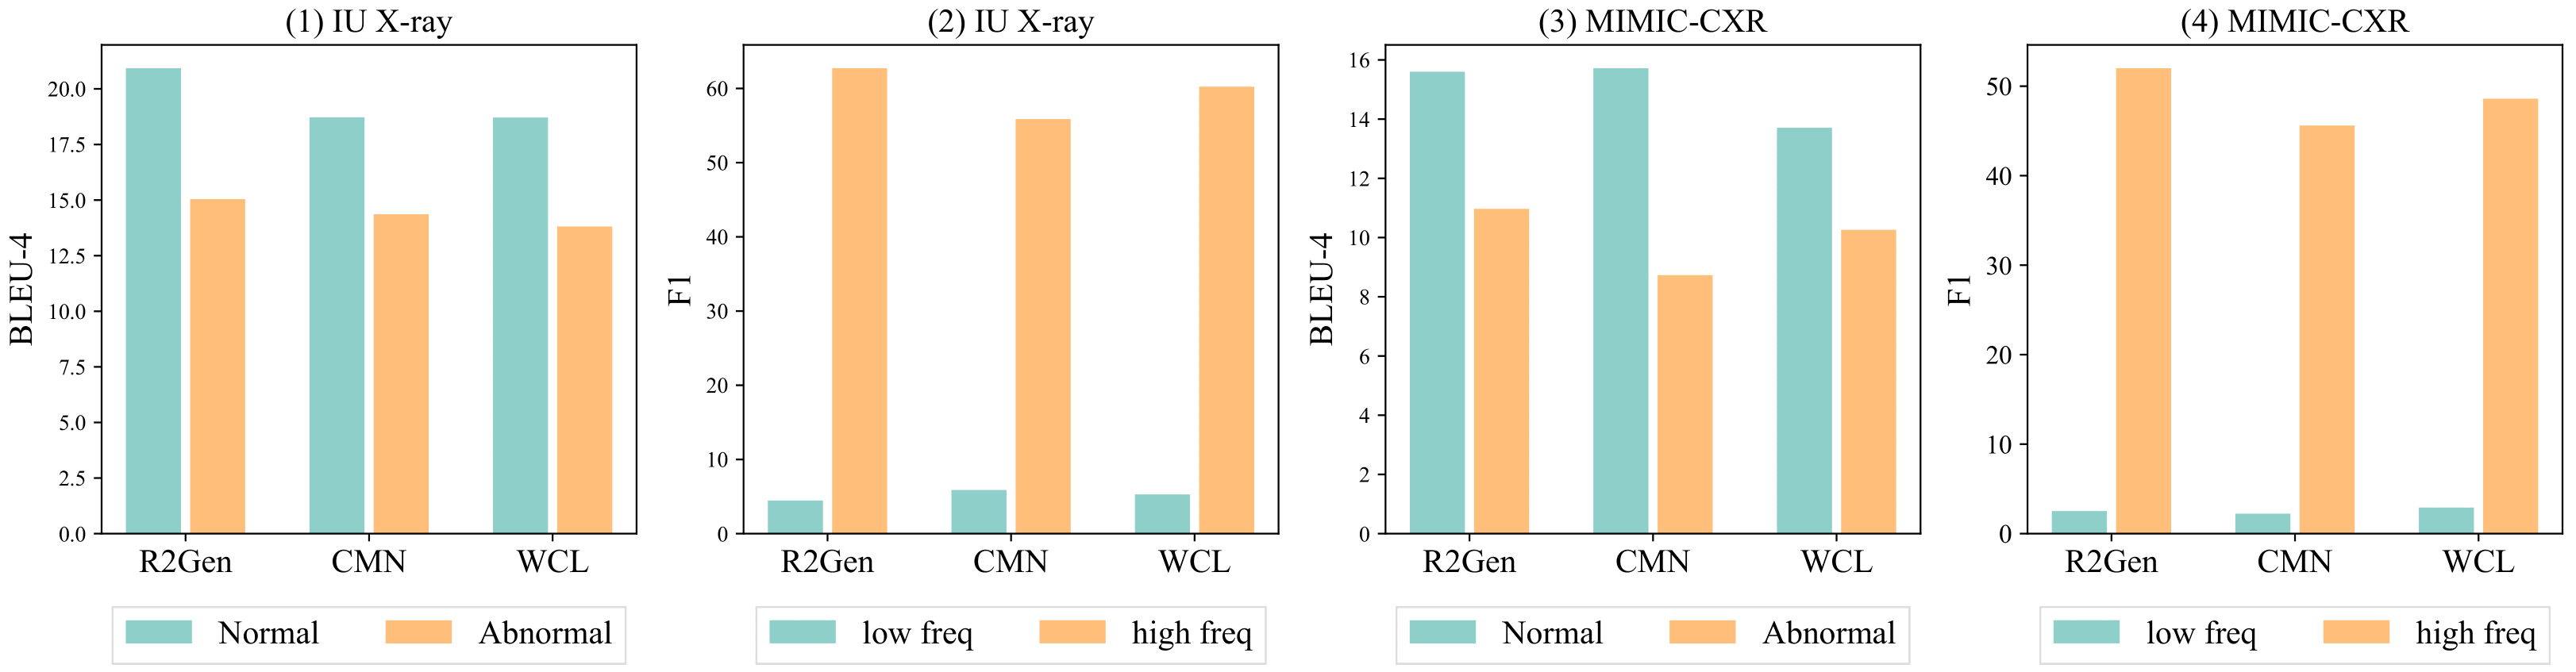
\includegraphics[width=0.95\textwidth]{image/label_im_performance.pdf}
\caption{State-of-the-art model performance on normal and abnormal entries by BLEU-4 (left two) and low- and high-frequent tokens by F1 scores (right two). \added[id=A]{We used two different colors to denote model performance on normal (orange) vs abnormal (light green) reports or frequent (orange) vs infrequent (light green) tokens.}}
\label{fig:label_im_performance}
\end{figure*}


Two major data imbalances exist in the radiology generation task, label and token. 
\textit{Label imbalance} pertains to a disproportionate ratio of normal and abnormal diagnosis categories, which exist in radiological images and text reports.
For instance, normal cases (images and reports) dominate radiology data, which can easily lead to underperformance in disease detection and professional description.
As shown in Table~\ref{tab:data}, abnormal reports are considerably longer than normal reports while can only count less than 15\%. 
These abnormal reports are much harder to generate than shorter reports~\cite{lovelace2020learning, tan2021progressive, wang2023metransformer} and can be worse with fewer samples than normal cases.\footnote{Clinical reports are also much longer than general-domain image captions, such as MS-COCO~\cite{lin2014microsoft}.}
Existing imbalance learning studies of radiology report generation primarily focus on label imbalance~\cite{nishino2020reinforcement, yu2022clinically}.
\textit{Token imbalance} is a critical challenge in generation that tokens have varied occurrence frequencies, and the issue is more critical in the medical task.
Learning infrequent tokens can be harder than frequent tokens for generation models~\cite{gu2020token,wu2023token}.
Medical tokens appear less frequently than regular ones, and the infrequent tokens may contain more medical results, highlighting the very unique challenge of this task.
\added[id=A]{The imbalance issue in radiology report generation also connects to broader challenges in multi-label classification or image object detection tasks, where models often struggle to effectively learn from infrequent but clinically significant labels~\cite{li2022survey} and object categories~\cite{lin2020focal}.}
Figure~\ref{fig:label_im_performance} illustrates the learning progress of the state-of-the-art (SOTA) model RRG~\cite{delbrouck2022improving} in predicting a report with predominantly normal diagnoses.
The model shows strong performance on normal cases but struggles on abnormal reports.


% \begin{figure}[htp]
% \centering 
% \caption{Models overfit on normal cases as abnormal patterns are infrequent.}
% \includegraphics[width=0.6\textwidth]{image/sample_prediction_crop (1).pdf}
% \label{fig:sample_prediction}
% \end{figure}


To promote the quality of generated reports, we propose \textbf{J}oint \textbf{Im}balance \textbf{A}daptation (JIMA) model by curriculum learning~\cite{bengio2009curriculum}\added[id=A]{, a training strategy to present models with increasingly complex examples and mimic human learning from simple to difficult task}.
JIMA automatically guides the model learning process by leveraging optimization difficulties, strengthening learning capability on infrequent samples, and alleviating overfitting on frequent patterns on both label and token.
\added[id=A]{Our method implements a tailored curriculum strategy dynamically adjusts data example difficulties by integrating radiology-domain-specific knowledge and difficulty metrics no previously considered in curriculum learning approaches, which aims to address data imbalance and promote radiology report quality.}
We incorporate the token and label metrics as a joint optimization and design a novel Training Scheduler that sampling and sorting training instances with a multi-aspect scoring mechanism.
The scheduler automatically adjusts training samples when model performance varies across multiple imbalance factors.
We conduct experiments on two publicly available datasets, MIMIC-CXR~\cite{johnson2019mimic} and IU X-ray~\cite{demner2016preparing} with automatic and human evaluations.
By comparing with six state-of-the-art (SOTA) baselines on overall and imbalance performance settings, our approach shows promising results over the SOTA baselines.
\added[id=A]{Notably, JIMA demonstrates minimal impact on the performance of highly frequent tokens and labels, significantly enhances performance for moderately frequent samples, and reveals limitations in boosting performance for the rarest tokens.}
Our ablation and qualitative analyses show that JIMA can generate more precise medical reports, alleviating label and token imbalance.
%Our code and data access will be available at [URL].

\section{Related Work}

\textbf{Radiology report generation} is a domain-specific image-to-text task that has two major directions, retrieval- \cite{endo2021retrieval, jeong2023multimodal} and generation-based \cite{chen2020generating, qin2022reinforced,kale2023replace}. 
The retrieval-based approach compares similarities between an input radiology image and a set of report candidates, ranks the candidates, and returns the most similar one~\cite{liu2021competence, endo2021retrieval, jeong2023multimodal, wang2023metransformer,delbrouck2023overview}. 
In contrast, our study focuses on the generation-based task, which automatically generates a precise report from an input image. 
The task has domain-specific characteristics in the clinical field. 
% As illustrated in Section~\ref{sec:data}, 
The clinical data contains many infrequent medical terminologies and longer documents than image captioning from general domains~\cite{lin2014microsoft}.
As radiology report generation can reduce the workloads of radiologists, generating highly qualified and precise can be a critical challenge, especially under the imbalance settings. %from Section~\ref{sec:data}.
Differing from previous work, we aim to promote model robustness and reliability under imbalance settings, which have been rarely studied in the radiology report generation.


\textbf{Imbalance learning} aims to model skewed data distributions. 
The primary focus of imbalance learning is on class or label imbalance, such as positive or negative reviews in sentiment analysis~\cite{li2022survey}.
\added[id=A]{
Recent studies have proposed new approaches to solve imbalance issues by weighting hard and infrequent examples~\cite{lin2020focal} or leveraging imbalance distributions to augment minority data labels~\cite{li2022survey, chawla2002smote}. 
The studies can inspire our work to model multiple imbalance factors, as the imbalance is a multifaceted issue in radiology report generation that exists beyond the data label.}
\sout{While previous studies proposed new objective functions (e.g., focal-loss~\cite{lin2020focal}) or oversampling~\cite{chawla2002smote}, those methods may not be applicable to our primary generation unit, token, which has large vocabulary sizes and extreme sparsity.}
\added[id=A]{Some studies developed new objective functions or data augmentation approach to promote model performance on minority labels, such as focal-loss by down-weighting easy samples~\cite{lin2020focal} or SMOTE by creating synthetic data on minority labels~\cite{chawla2002smote}.
However, those methods may not be applicable to our primary generation unit, token, which has large vocabulary sizes and extreme sparsity.}
In terms of radiology report generation, reports may have disease-related labels.
Recent studies have augmented model robustness by balancing performance between disease and normal by reinforcement learning~\cite{nishino2020reinforcement, yu2022clinically}.
\sout{However, those methods ignore a fundamental challenge of generation task, token imbalance -- a long-tail distribution.}
\added[id=A]{However, those methods focused on the label imbalance, and our study considers a multifaceted imbalance challenge, including label and token imbalance.}
The token imbalance can be even more critical for the clinical domain, as medical tokens appear less frequently than regular tokens in radiology reports.
\added[id=A]{A close work is the TIMER~\cite{wu2023token}, which considers the token imbalance. However, the approach ignores other imbalance factors, which is solved by our approach. Particularly, our approach jointly models multiple imbalance factors, label and token, and we propose a new curriculum learning method to learn the imbalance factors.}
\sout{Our study makes \textit{a unique contribution} to the radiology report generation that jointly consider multiple imbalance factors via curriculum learning.}


\section{Data}
\label{sec:data}

We collected two publicly accessible datasets for this study, IU X-ray~\citep{demner2016preparing} and MIMIC-CXR~\cite{johnson2019mimic}, de-identified chest X-ray datasets to evaluate radiology report generation.
IU X-ray~\citep{demner2016preparing}, collected from the Indiana Network for Patient Care, includes 7,470 X-ray images and corresponding 3,955 radiology reports.
MIMIC-CXR~\citep{johnson2019mimic}, collected from the Beth Israel Deaconess Medical Center, contains 377,110 X-ray images and 227,827 radiology reports for 65,379 patients.
Each report is a text document and associates with one or more front and side X-ray images.
Table~\ref{tab:data} summarizes statistics of data imbalance and Figure~\ref{fig:label_imbalance} visualize the distributions of frequent (ranked in the top 12.5\% of the vocabulary) and infrequent tokens.
We include preprocessing details in Appendix~\ref{appendix:sec:data}.

\begin{table*}[t]
    \centering
    %We report the size of radiology image, report, and vocabulary.
    \caption{Data statistics summary. Variations exist in label (Normal and Abnormal \%) and average report length ($L$). \added[id=A]{Vocab refers to the vocabular size, and normal or abnormal indicates report labels.}}
    \resizebox{.99\textwidth}{!}{
    \begin{tabular}{c|c|c|c|c|c|c|c|c}
    & Image & Report & Vocab & Abnormal \% & Normal \% & $L$ & $L_{normal}$ &$L_{abnormal}$\\\hline\hline
    IU X-ray &7,470 &3,955 &1,517 &32.96\% & 67.04\% &35.99 &27.76 &40.72\\
    MIMIC-CXR  &377,110 &227,835 &13,876  &13.97\% &86.03\% &59.70 &34.57 & 59.36\\
    \end{tabular}
    }
    \label{tab:data}
\end{table*}

Table~\ref{tab:data} presents imbalance patterns in tokens and labels.
Abnormal entries are predominant in both datasets, and MIMIC-CXR displays a more skewed label distribution, as more abnormal samples were collected during diagnosis phases not for screening purposes.
MIMIC-CXR has a longer average length than IU X-ray. 
The lengthier documents may pose a unique multimodal generation challenge in the medical field. 
To conduct our analysis, we define the low and high frequency using the top 12.5\% frequent tokens. 
Figure~\ref{fig:label_im_performance}  suggests a joint relation between label and token imbalance and higher ratios of low-frequency tokens in abnormal reports.
This observation motivates us to investigate how the imbalance impacts model robustness and reliability.


\subsection{Imbalance Effects}
\begin{figure}[htp]
    \centering 
    \caption{Frequent and infrequent token distributions conditioning on report label. \added[id=A]{We denote the report types with light green (normal) and orange (abnormal), which show different token imbalance distributions.}}
    \includegraphics[width=0.7\textwidth]{image/data_label_imbalance.pdf}
    \label{fig:label_imbalance}
\end{figure}

We examine the potential impact of label and token imbalance on model performance. 
To ensure consistency, we keep the top 12.5\% to split low- and high-frequent tokens for evaluation purposes.
The analysis includes three state-of-the-art models, R2Gen~\citep{chen2020generating}, WCL~\citep{yan2021weakly}, and CMN~\citep{chen2021cross}.
% We either use released source codes and leave implementation details in the Appendix~\ref{sec:implementation}.
We use BLEU-4~\citep{papineni2002bleu} and F1 scores to measure performance across both token (low vs high frequency) and label (normal vs. abnormal) imbalance. 
We visualize performance variations in Figure~\ref{fig:label_imbalance}.


The results suggest that the models exhibit significant difficulties in coping under label and token imbalance.
Models consistently perform worse on abnormal reports, which are lengthier and have more infrequent tokens than normal reports. 
For example, the top 12.5\% frequent tokens count $>$ 80\% tokens in two datasets, and low-frequent tokens have much worse performance than frequent tokens, as infrequent tokens are harder to optimize~\citep{yu2022rare}.
However, infrequent tokens contain higher ratios of medical terms (e.g., silhouettes and pulmonary) describing health states.
The significantly varying performance highlights the unique challenges to adapt token and label imbalance.
While existing work~\citep{nishino2020reinforcement} has considered label imbalance, however, the study did not examine the performance effects of label or token imbalance.
The findings inspire us to propose our model \textbf{J}oint \textbf{Im}balance \textbf{A}daptation (\textit{JIMA}) to model token and label imbalance.


\section{Joint Imbalance Adaptation}

In this section, we present our approach \textbf{J}oint \textbf{Im}balance \textbf{A}daptation (\textit{JIMA}) in Fig~\ref{fig:mr} by using \textit{curriculum learning}.
JIMA aims to augment model robustness under label and token imbalance.
As optimizing data imbalance has been demonstrated difficulty, deploying such a learning strategy will strengthen model robustness and reliability.
Our proposed approach deploys curriculum learning (\textit{CL})~\cite{wang2022survey} that automatically adjusts the optimization process by gradually selecting training data entries from learning difficulty --- learning from hard to easy samples as our optimization strategy~\cite{zhou2020advances}.
To achieve the goal, we design two major CL modules, difficulty measurer for assessing the difficulty of samples, and a training scheduler for determining the percentage of training data.
Then we employ our CL training strategy to two tasks. 
Task 1 aims to predict entities from the images and Task 2 can generate a report from images' features and entity distribution.

\begin{figure*}[htp]
    \label{overview}
    \centering
    \caption{JIMA has two \added[id=A]{curriculum learning} tasks. Task 1 aims to predict entity distribution from images, and task 2 aims to generate report from image's feature and entity distribution. We assign one color per task and solid arrows as workflows. \added[id=A]{We extracted imbalanced entity distributions from the training data by the Radgraph as the gold truth and compare the entity estimation with the predicted entity distribution. We feed the fused radiology image features and imbalance patterns for the generation process. During the training, the task 1 and 2 decide which data samples will be fed for the model training.}}
    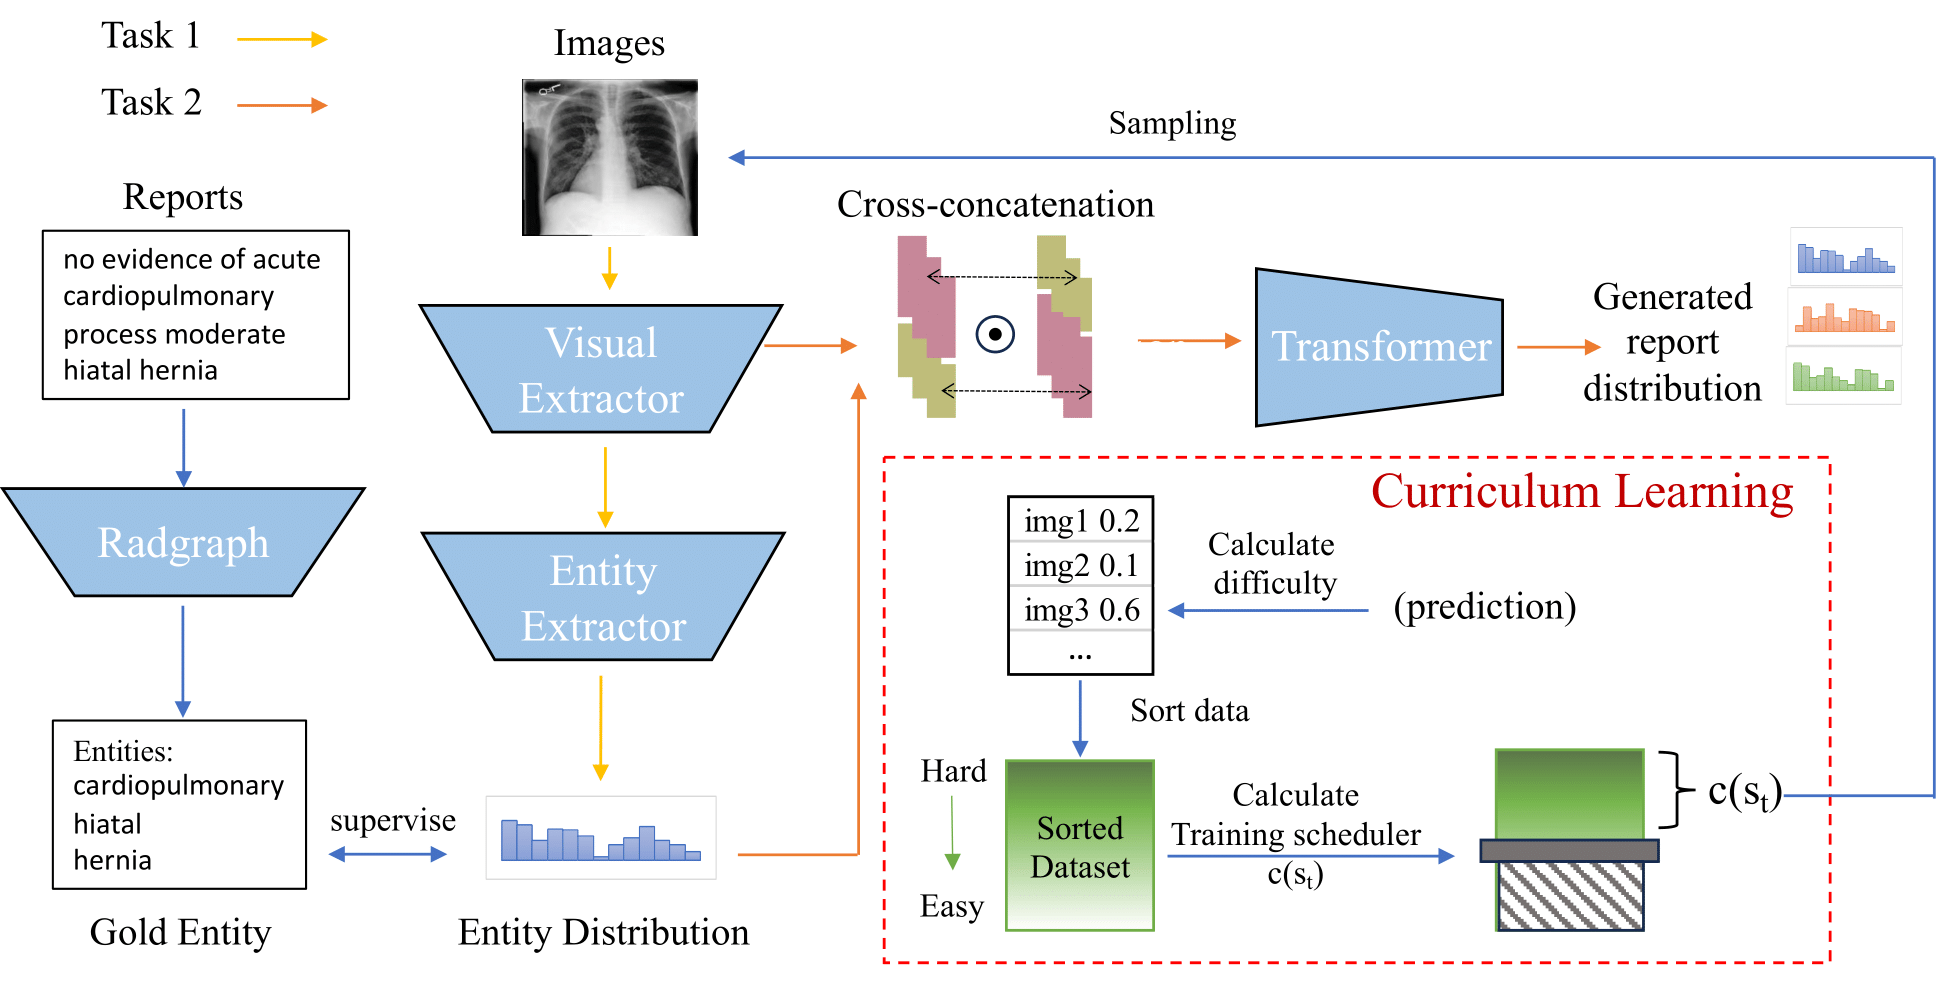
\includegraphics[width=0.99\textwidth]{image/crop_acl2024_overview.pdf}
    \label{fig:mr}
\end{figure*}


\textit{Difficulty measurer} is \added[id=A]{the core scoring function of the curriculum learning that decide which data samples should be fed to models for training.}
To diversify learning aspects and jointly incorporate imbalance factors, we propose a novel measurement to improve model performance over imbalance patterns. 
Our measurement adopts a competitive mechanism that encourages correct options with higher ranking over incorrect ones, rather than independently increasing the likelihood of correct options and decreasing the likelihood of incorrect options. This approach helps mitigate overfitting on common samples and underfitting on rare samples since it focuses on ranking of correct option rather than prediction confidence.
Specifically, given a reference token $z$, vocabulary list $V$ and the prediction $\mathbf{p} \in \mathcal{R}^{|V|}$, we calculate the token reference ($z$) probability ranking in the prediction $\mathbf{p} $ as the following,
\begin{equation}\label{eq:Difficulty}
    k = Rank(\mathbf{p}, \mathbf{p}[z])/ |V|
\end{equation}
where $|V|$ is the vocabulary size. 
$Rank(\mathbf{p}, \mathbf{p}[z])$ assigns a rank to $\mathbf{p}$ in descending order and identifies the position of $\mathbf{p}[z]$ within this ranking.
\added[id=A]{We used the $Rank()$ function to inference imbalance distributions on the token level, which will give a higher preference towards tokens that are hard to predict. To avoid the biased performance evaluation in different labels and tokens, we calculate the average value in non-entity and entity tokens separately, extracted by the Radgraph~\cite{jain2021radgraph}.}
%To avoid the biased performance evaluation in different labels and tokens, we calculate the average value in non-entity and entity tokens separately.
$k$ ranges from $0$ to $1$ under regularization with $|V|$. A higher value of $k$ indicates that the sample is more difficult.
Then, we feed the difficulty information to the next step, Training Scheduler.

% Next, we employ our curriculum learning patterns introduce above to improve labels robustness by task 1 and tokens robustness by task 2.
\textit{Training scheduler} aims to automatically leverage imbalance effects by selecting training samples via the difficulty measurers.
Our goal is to increase the number of easier samples when the performance decreases and vice versa. 
According to our goal, we design our scheduler function, $c(s_{t})$ as following: 
\begin{equation}\label{sampling}
    c(s_{t}) = min(1, [1-\frac{(s_{t}-s_{t-1})}{s_{t-1}}] \times c(s_{t-1})), t \geq 1
\end{equation},
where $s$ is the average performance of all training samples, measuring the model's learning ability. $t$ is the training step.
% TODO Yuexin
Given decreasing performance as an example, $\frac{(s_{t}-s_{t-1})}{s_{t-1}}$ will be negative.
During the process, the ratio $1-\frac{(s_{t}-s_{t-1})}{s_{t-1}} > 1$ will allow the model to include more easy training data than the last step $c(s_{t-1})$. 
When the performance increase, the scheduler feed less easy samples to the model and reduce the over-fitting on these samples.
After multiple epochs of training, harder samples  receive more training iterations than easier samples.
In this way, we can alleviate the the challenge from imbalanced tokens and labels in radiology report generation task.
To start our curriculum learning, we record the samples' average performance of the last two regular training epochs as $s_{0}$ and $s_{1}$, where we empirically initialize $c(s_{0})$ as 1.



\subsection{CL-Task 1}
\label{subsec:task1}
CL-Task 1 is to exploit imbalance patterns of radiology labels to generate clinically accurate reports. 
Entities in clinical reports play a crucial role in disease diagnosis. 
However, these clinical tokens often occur infrequently and are significantly underestimated during model training. 
Hence, we assess the accuracy of clinical entities to evaluate performance.
Our intuition is that as abnormal cases contain more infrequent entities, focusing on the clinical entities may benefit the abnormal cases.
If our generated reports are clinically correct, the visual extractor can accurately extract the same entities as gold entities from images.
% We utilize a binary label schema to keep consistency across IU X-ray and MIMIC-CXR. In IU X-ray, we use the labels provided by Medical Subject Heading (MESH), which is a binary value (normal or abnormal).  In MIMIC-CXR, we use CheXbert to extract samples' labels and binarize the predicted labels (no findings vs other 13 diseases). 
%In order to assess the difficulty level of each sample, we utilize F1 score, which reflects the degree of agreement between the predicted and true labels. 
%The greater the discrepancy between the predicted and true labels indicates harder samples and vice versa. 
%As clinical performance is a critical metric for radiology report generation, we utilize clinical error to sample data for Task 1.
% First, we train a classifier for IU X-ray. 
%We expect this task helps the model leverage label imbalance, as the training scheduler can strengthen model training on the misclassified samples.


The computing process is as the following. 
%First, we extract the gold entities from reference reports by radgraph~\cite{jain2021radgraph}.
Given a radiology image $Img$ and the corresponding report $Z =\left(z_{0}, \ldots, z_{l}\right)$ with the length $l$, we extract the features from images with a visual extractor. 
We use ResNet101~\cite{he2016deep} ($f_{\mathcal{R}}$) as our visual extractor and obtain image features ($\mathbf{X}$) from different convolutional channels, $\mathbf{X} = f_{\mathcal{R}}(\operatorname{Img})$.
$\mathbf{X} \in \mathcal{R}^{patch\_size \times d}$, where $d$ is the size of the feature vector.
To predict entities distribution, we feed the feature from $\mathbf{X}$ into the Entity Extractor ($f_{E}$) with parameters $W_{E} \in \mathcal{R}^{d \times |V|}$ and average the value on each patch(1st dimension), 
\begin{equation}\label{entity distribution}
   \mathbf{q} = AVG_{:1}(f_{E}(\mathbf{X} | W_{E}))
\end{equation}
Then we obtain the entity distribution representation $\mathbf{q} \in  \mathcal{R}^{|V|}$. 
To optimize the model,  we minimize Binary Cross Entropy as follows,
 \begin{equation}\label{eq:nll}
    \mathcal{L}_{task1} = \frac{1}{|V|} \sum_{i=1}^{|V|}-\left(y_i{ }^* \log \left(q_i\right)+\left(1-y_i\right) * \log \left(1-q_i\right)\right)
 \end{equation}
 where $q_{i}$ is the prediction probability of the i-th token and $y_{i} = 1$ if i-th token is the entities. We extract the gold entities ($\mathbf{e}$) by radgraph~\cite{jain2021radgraph}.
To evaluate sample's difficulty in this task, we input the entity distribution prediction $\mathbf{q}$ into e.q~\ref{eq:Difficulty} and obtain
    $k^{task1} = \sum_{i}^{|\mathbf{e}|} Rank(\mathbf{q},\mathbf{q}[e_{i}])/( |V| \cdot |\mathbf{e}|)$.


%Samples containing infrequent tokens are prone to obtaining lower F1 scores, and as such, the samples will be prioritized in training data repeatedly. 
%This approach allows the model to devote more attention to learning from samples containing infrequent tokens, particularly when the model struggles to capture the underlying patterns in such tokens.
%Since infrequent tokens have much higher ratios of medical terms, leveraging token imbalance will be beneficial.

 %We get $s_{i}$  from $\mathcal{Q}$ in task 1 and $\mathcal{K}$ in task 3.
% Generally, each task manages different module parameters optimization. 
% The model learns images' feature representation from the simple task (task2) and learns to generate from the difficult tasks (task1 \& task3).


\subsection{CL-Task 2}
%写如何adapt to token imabalance. 只是预测distribution 不包含frenquency. samples with more rare tokens have a greater loss.
%Inspired by the idea of curriculum learning, we start to train our model with a simple task. 
% TODO: Yuexin write a description similar to the 1st paragraph in the Task 1.
%The objective of Task 2 is to exploit token imbalance by predicting word occurrences in a given report. 
% In contrast to the text generation task, the process does not account for word order and involves irrelevant-sequence prediction.
%We utilize a multi-class binary schema to denote the tokens' occurrence and calculate the token F1 score as the difficult metrics. 
%This approach does not count the tokens' frequency and assigns the same weight to all tokens.
%As a result, samples with infrequent tokens are identified as difficult and can be used by the training scheduler to enhance the model's performance in handling rare tokens.
CL-Task 2 implements an image-to-text generation pipeline with the objective of improving the infrequent tokens prediction in reports.
To generate a report containing more clinically useful information, we integrate the probability prediction of entities($\mathbf{q}$) in e.q.~\ref{entity distribution} with image's feature ($\mathbf{X}$).
Since $d \neq |V|$, we cannot interact $\mathbf{q}$ and $\mathbf{X}$ directly. To facilitate their interaction and information sharing, we employ a cross-concatenation and perform \sout{a dot product}\added[id=C]{an element-wise multiplication} operation on their cross-concatenated matrix as follows:
\begin{equation*}
     \mathbf{S} = concat_{:2}(\mathbf{X}, \mathbf{q}) \odot concat_{:2}(\mathbf{q}, \mathbf{X})
\end{equation*}, where $\mathbf{S} \in \mathcal{R}^{patch\_size \times (d + |V|)}$ \added[id=C]{and $\odot$ refers to the element-wise multiplication}. \added[id=C]{We empirically compare with simple sum, dot product, and cross-modal attention network~\cite{song2022cross}; however, the element-wise multiplication achieved the best results on the validation set.
We infer that the multiplication is less complex than the cross-modal attention network while keeps more vector information from the text and image modalities.}
Finally, we adopt a transformer structure to encode $\mathbf{S}$ and generate i-th token probability distribution $\mathbf{P_{i}}$ from encoding feature $\mathbf{S}$ and i-th token, $\mathbf{{P}_{i}}  =  f_{{\mathcal{T}}}(\mathbf{S}, z_{i-1})$.
To optimize the model,  we minimize negative log-likelihood loss (NLL) as follows,
\begin{equation}
    \mathcal{L}_{task2} =  -\sum_{i}^{l} \log \left(\mathbf{P_{i}}\right) 
\end{equation}
We can access the sample's difficulty with $\mathbf{P_{i}}$ by e.q.~\ref{eq:Difficulty}, 
 $k^{task2} = \sum_{i}^{l} Rank(\mathbf{P}_{i},\mathbf{P}_{i}[z_{i}])/( |V| \cdot l) $.
 

\begin{algorithm}
 \caption{Optimization Process of JIMA}
 \label{alg:Framwork}
 \begin{algorithmic}[1]
     \Require  Learning rate $\alpha, \beta $
     \For {each epoch}
      \State Rank entries by the two difficulty measurers ($k^{task1}$ and $k^{task2}$), and obtain two sorted datasets $\mathcal{D}_{1}$, $\mathcal{D}_{2}$
     \State Calculate $c(k_{t}^{task1})$ and $c(k_{t}^{task2})$ training schedulers
     \State Select top $c(k_{t}^{task1})$ samples from the sorted datasets $\mathcal{D}_{1}$ obtained by step 1 as training sets
      \State Select top $c(k_{t}^{task2})$ samples from the sorted datasets $\mathcal{D}_{2}$ obtained by step 1 as training sets
     \State Sample a batch from $\mathcal{D}_{1}$ and update Task 1:
     $\widetilde{f}_{\mathcal{R}}\gets f_{\mathcal{R}}-\alpha\nabla_{f_{\mathcal{R}}}\mathcal{L}_{task1}$, $\widetilde{f}_{E}\gets f_{E}-\alpha\nabla_{f_{E}}\mathcal{L}_{task1}$
     \State Sample a batch from $\mathcal{D}_{2}$ and update Task 2:
    $\widetilde{f}_{\mathcal{T}}\gets f_{\mathcal{T}}-\beta\nabla_{f_{\mathcal{T}}}\mathcal{L}_{task2}$
     \EndFor
\end{algorithmic}
\end{algorithm}


\subsection{CL-Joint Optimization}
We propose a joint optimization approach to integrate two tasks. 
Algorithm~\ref{alg:Framwork} summarizes the overall optimization process of our approach.
We set the learning rate of task 1 as $\alpha$ and $\beta$ refers to the learning rate of tasks 2.
In each training step, we sample different data for different tasks and each task focuses on optimizing its own module of the models. 
For example, we update the visual extractor ($f_{\mathcal{R}}$) and the entity extractor ($f_{E}$) in task 1. 
Next, we freeze the parameters of the visual extractor and the entity extractor, and update the parameters of the transformer ($f_{\mathcal{T}}$) specifically for task 2.
 Our optimization approach integrates with curriculum learning to tailor joint imbalance learning for each module ($f_\mathcal{R}$, $f_{E}$, $f_\mathcal{T}$, ). Curriculum learning empowers the model to concentrate on optimizing hard samples while mitigating the risk of overfitting to easier samples. The joint optimization scheme facilitates  each task to manage different module parameters optimization and learn a transferable knowledge from the simpler to more complex task. As a result, all modules collaborate to enhance error reduction from previous tasks.


\section{Experiments}

We design our experiments to evaluate performance on both regular and imbalanced settings via automatic and human evaluations. 
The automatic evaluation includes NLG-oriented and clinical-correctness metrics.
NLG-oriented metrics measure the similarity between generated and reference reports. 
Clinical correctness and human evaluation belong to factually-oriented metrics, and domain-specific evaluation methods. 
To be consistent with our baselines~\cite{chen2020generating, delbrouck2022improving, wu2023token}, we utilize the F1 CheXbert~\cite{smit2020combining} for the clinical-correctness metrics. 
The experiments compare our proposed approach (JIMA) and the state-of-the-art baselines. 
Two of our five baselines (CMM + RL \& RRG) are designed to solve label imbalance by improving the abnormal findings generation. 
We conduct ablation and case analyses to fully understand the capabilities of our proposed approach.
We include more implementation details and hyperparameter settings in Appendix~\ref{sec:implementation}.


\subsection{Baselines}
\label{subsec:baselines}
To examine the validity of our method, we include five state-of-the-art baselines under the same experimental settings:
%Transformer~\cite{vaswani2017attention}, 
R2Gen~\cite{chen2020generating}, CMN~\cite{chen2021cross}, WCL~\cite{yan2021weakly}, CMN + RL~\cite{qin2022reinforced}, RRG~\cite{delbrouck2023overview}, TIMER~\cite{wu2023token} and RGRG~\cite{tanida2023interactive} -- and obtain from their open-sourced code repositories.

\textbf{R2Gen}~\cite{chen2020generating} is a transformer-based model with ResNet101~\cite{he2016deep} as the visual extractor. To capture some patterns in medical reports, R2Gen proposes a relational memory to enhance the transformer so that the model can learn from the patterns' characteristics.  Furthermore, R2Gen deploys a memory-driven conditional layer normalization to the transformer decoder facilitating incorporating the previous step generation into the current step.
    
\textbf{CMN}~\cite{chen2021cross} is a novel extension to the transformer architecture that facilitates the alignment of textual and visual modalities. The cross-modal memory network record the shared information of visual and textual features. The alignment process is carried out via memory querying and responding. The model maps the visual and textual features into the same representation space in memory querying and learns a weighted representation of these features in memory responding.

\textbf{WCL}~\cite{yan2021weakly} utilizes the R2Gen framework and incorporates a weakly supervised contrastive loss. Specifically, WCL leverages the contrastive loss to enhance the similarity between a given source image and its corresponding target sequence. Furthermore, the model enhances its ability to learn from difficult samples by assigning more weights to instances sharing common labels.

\textbf{CMM + RL}~\cite{qin2022reinforced} is a cross-modal memory-based model with reinforcement learning for optimization. CMM + RL designs a cross-modal memory model to align the visual and textual features and deploy reinforcement learning to capture the label imbalance between abnormality and normality.
The author uses BLEU-4 as a reward to guide the model to generate the next word from the image and previous words. 
%proposes a method for aligning text and image features over a cross-modal memory using reinforcement learning. Upon generating the end-of-sequence (EOS) token, reward the generation model based on evaluation metrics.

\textbf{RRG}~\cite{delbrouck2022improving, delbrouck2023overview} aims to generate clinically correct reports by weakly-supervised learning of the entities and relations from reports. RRG is a BERT-based model with Densenet-121~\cite{huang2017densely} as a visual extractor. RRG leverages RadGraph~\cite{jain2021radgraph} to extract the entities and relation labels in a report. RRG utilizes reinforcement learning to optimize the model. The reward assesses the consistency and completeness of entities and the relation set between generated reports and reference radiology reports. RRG addresses label imbalance issues by maximizing the reward of predicting more complicated entities and relations in abnormal samples.

\textbf{TIMER}~\cite{wu2023token}  aims to decrease the over-fitting of frequent tokens by introducing unlikelihood loss to punish the error on these tokens. The tokens set of unlikelihood loss is automatically adjusted by maximizing the average F1 score on different frequency tokens. 

\textbf{RGRG}~\cite{tanida2023interactive} adopts GPT2 as  the language generation model and generate a report based on the localized visual features of anatomical regions, which are extracted by a object detection.
This baseline experiment was specifically carried out on the MIMIC-CXR dataset, as the IU X-ray dataset lacks anatomical region information, resulting in the inability to train an object detection module effectively.

% Detailed baseline implementations are in the Appendix~\ref{sec:implementation}.


\subsection{Imbalance Setting}
\label{subsec:im_sec}
We evaluate model robustness under token and label imbalance settings and present results in Section~\ref{subsec:imb_tok_perf} and \ref{subsec:label_imb_perf}. 
For token imbalance, we compare F1-scores of frequent and infrequent tokens separately. 
We introduce three different scales to define frequency token sets, $1/4$, $1/6$, and $1/8$ respectively.
The splits define the top $1/4$, $1/6$, and $1/8$ vocabulary as frequent tokens and the rest vocabulary as infrequent tokens. 
The setting is to demonstrate the effectiveness of our approach in adapting token imbalance. 
For label imbalance, we divide our samples into a binary category, normal and abnormal. 

\section{Results and Analysis}
\begin{table*}[htp]
    \centering
    \caption{Overall performance. $\overline{\Delta}$ is the averaged percentage improvements over baselines, \added[id=A]{and the $\hat{\Delta}$ refers to the percentage improvements over the state-of-the-art model. The evaluation include both generation (NLG) and clinical-correctness (CE) metrics, where bolden numbers indicate the best performance.}}
    \label{tab:overall_performance}
    \resizebox{.99\textwidth}{!}{
    \begin{tabular}{c|c|c|c|c|c|c|c|c}
        \multirow{2}{*}{Dataset} & \multirow{2}{*}{Model} & \multicolumn{6}{c|}{NLG metrics} & CE metrics \\ 
         &~ & BLEU-1 & BLEU-2 & BLEU-3 & BLEU-4 & METEOR & ROUGE-L & F1 \\ \hline\hline
        \multirow{8}{*}{IU X-ray}& R2Gen & 48.80 & 31.93 & 23.24 & 17.72 & 20.21 & 37.10 &63.62 \\ 
        ~ & CMN & 45.53 & 29.50 & 21.47 & 16.53 & 18.99 & 36.78 &64.83\\ 
        ~ & WCL & 44.74 & 29.30 & 21.49 & 16.79 & 20.45 & 37.11 &49.24 \\ 
        ~ & CMM + RL & 49.40 & 30.08 & 21.45 & 16.10 & 20.10 & 38.40 &40.79 \\ 
        ~ & RRG &49.96 &31.44 &22.11  &17.05   &18.81  &33.46 &49.10\\
        ~ &TIMER & 49.34 & 32.49 & 23.84 & 18.61 &20.38 &38.25 &94.52\\
        ~ & JIMA (Ours) & \textbf{50.50} & \textbf{33.12} & \textbf{24.15} & \textbf{18.88}  & \textbf{21.16} & \textbf{38.56} & \textbf{96.58}  \\ \hhline{~|--------}
        ~ &\added[id=B]{$\overline{\Delta}$ (\%)} &5.49  &7.74 &8.65 &10.44 &6.86 &4.86 &72.10\\
        ~ &\added[id=B]{$\hat{\Delta}$ (\%)} &2.35  &1.93 &1.30 &1.45 &3.82 &0.81 &2.18\\\hline
        \multirow{8}{*}{MIMIC-CXR} & R2Gen & 35.42 & 21.99 & 14.50 & 10.30 & 13.75 & 27.24 &54.60  \\ 
        ~ & CMN & 35.60 & 21.41 & 14.07 & 9.91 & 14.18 & 27.14 &50.50  \\ 
        ~ & WCL & 37.30 & 23.13 & 15.49 & 10.70 & 14.40 & 27.39 &55.58  \\ 
        ~ & CMM+RL &35.35	&21.80	&14.82	&10.58	&14.20	&27.37 &65.43 \\ 
        ~ & RRG &37.57 &19.78 &15.87 &9.56 &14.77 &26.81 &62.20\\
        ~&TIMER & 38.30 &22.49 & 14.60 & 10.40 &14.70 & 28.00 &75.86\\
        ~& RGRG &30.7	&20.59	&14.10	&10.18	&15.43	&24.03 &80.28\\
        ~ & JIMA (Ours) &\textbf{41.37}	&\textbf{24.83} &\textbf{16.72}	&\textbf{11.20}	&\textbf{16.75} &\textbf{30.15}	&\textbf{81.25} \\ \hhline{~|--------}
         & \added[id=B]{$\overline{\Delta}$(\%)} &16.26&	15.24	&13.34 &9.59	&15.73&	12.52&	31.29\\
         ~ &\added[id=B]{$\Hat{\Delta}$(\%)} &8.02 &10.40 &14.52 &7.69 &13.94 &7.68 &1.21\\
    \end{tabular}
    }
\end{table*}


% 
% We report performance and present analysis.
In this section, we present overall performance and report results of imbalance evaluations and include an ablation analysis and a case study.
% Appendix~\ref{sec:case_study}.
Generally, JIMA outperforms the state-of-the-art baselines by a large margin, especially under imbalance settings.
Our qualitative studies show our method can achieve more clinically accuracy and generate more precisely clinical terms.



\subsection{Overall Performance}

Table~\ref{tab:overall_performance} presents the performance of JIMA by NLG and clinical-correctness metrics.
JIMA outperforms baseline models (both imbalance and regular methods) on BLEU scores by a large margin, confirming the validity of selecting training samples by our curriculum learning method.
The approach enables the model to learn multiple times from the samples with lower BLEU-4, resulting in a better performance compared to the baseline models.
For example, JIMA shows an improvement of 16.59\% on average for IU X-ray and 16.28\% for MIMIC-CXR.
We infer this is as our task 1 and 2 jointly work to improves the token and label imbalanced problem. 

Second, our model achieves the best performance in F1 of the clinical metric, which indicates the Task 1 (Section~\ref{subsec:task1}) can enable the model to put more attention on difficult samples with lower F1 scores. 
Additionally, our method promotes clinical token prediction as performance on infrequent tokens and medical terms have been improved. 
For example, our generation significantly outperforms the baselines on F1 score by 72.10\% on IU X-ray and 31.29\% on the MIMIC-CXR average. CMN $+$ RL performs better than other baselines on IU X-ray but not on MIMIC-CXR.
JIMA maintains a stable performance on both IU X-ray and MIMIC-CXR.
We infer this as our joint imbalance adaptation can yield more improvements.

\begin{table*}[htp]
\centering
\caption{Results on high- and low-frequent tokens with three ratio splits. \added[id=A]{We measured the model performance on frequent and infrequent tokens by F1-score.}}
% We define three ratio splits for diverse evaluations. For example, 1/8 represents the top 1/8 frequent tokens as a high-frequency set.
\label{tab:im}
    \begin{tabular}{cccccccc}
    && \multicolumn{2}{c}{IU X-ray} & \multicolumn{2}{c}{MIMIC-CXR} \\
     Ratio & Method & infreq & freq & infreq  & freq  \\\hline\hline
    \multirow{7}{*}{1/8} &R2GEN &4.46 &\textbf{62.73} &2.52 &52.01 \\
    &CMN  & 5.88 & 55.86 & 2.23 & 45.60 \\
    &WCL	&5.29	&60.23 & 2.91	&48.60 \\
    &CMN + RL	&5.19	&49.36 & 0.21	&23.64\\
    &RRG  &7.28 &41.94  &2.50 &43.57\\
     &TIMER &13.23 & 61.89 & 3.15 & 52.66\\
     &RGRG &- &-  &0.22 &31.33\\
    &JIMA (ours) &\textbf{14.87} &62.55 &\textbf{3.58} &\textbf{53.06}	 \\\hline
    \multirow{7}{*}{1/6}&R2GEN &2.80 &61.62 &2.02 &49.86\\
    &CMN  &5.75 & 65.12	&0.85 & 52.02 \\
    &WCL	&3.72	&59.26 &2.13	&47.88  \\
    &CMN + RL	&5.19	&49.36 & 0.14 &23.36\\
    &RRG  &4.55  &40.46 &2.09 &43.56 \\
    &TIMER  &5.93 & 67.79 &2.02 &51.72\\
     &RGRG &- &- &0.26 &30.66\\
    &JIMA (ours) &\textbf{10.52} &\textbf{68.82} &\textbf{2.83} &\textbf{52.32}\\\hline
    \multirow{7}{*}{1/4} &R2GEN &1.16 &59.98  &0.00  &48.77\\
    &CMN  &2.60 & 63.92 &0.33 &51.09 \\
    &WCL	&1.50	&56.83 &0.30	&46.95 \\
    &CMN + RL	&5.19	&49.36 & 0.07	&23.05\\
    &RRG  &2.04 &38.84 &0.39  &41.45 \\
     &TIMER & 8.66 & 64.00 & 0.58 & 51.39  \\
      &RGRG &- &-  &0.20 &29.56\\
    &JIMA (ours) &\textbf{9.77} &\textbf{66.23} &\textbf{0.94} &\textbf{51.92}\\
    \end{tabular}
\end{table*}


\subsection{Token Imbalance} 
\label{subsec:imb_tok_perf}
Table~\ref{tab:im} compares high- and low-frequent tokens F1 in different ratio splits. 
Our method consistently outperforms baselines in the low-frequent tokens across frequency splits ($\frac{1}{4}, \frac{1}{6}$, and $ \frac{1}{8}$) on IU X-ray and MIMIC-CXR.
While RRG and CMN + RL approaches have adapted label imbalance, the approaches may not be able to adapt the token imbalance.
Our approach achieves better performance on the token imbalance. 
%and comparatively better on the frequent sets.
%\vspace{-.5cm}
% \begin{table}[htp]
%     \centering
%     \caption{Ablation analysis. }\label{ab}
%     \begin{tabular}{c|cccc|ccccc}
%         \multirow{2}{*}{Metrics}&\multicolumn{4}{c|}{IU X-ray} & \multicolumn{4}{c}{MIMIC-CXR} \\
%         ~ & -task1 & -task2 & -task3 & full&  -task1 & -task2 & -task3 & full \\ \hline\hline
%         BLEU-1 &\textbf50.65  &48.82  &50.44 &50.50 &37.66  &34.58  &37.77 &\textbf{37.85 \\ 
%         BLEU-2 &31.64  & 31.28 &\textbf{32.56 & 32.08 &\textbf{23.30  &22.58  &22.86 &23.26\\ 
%         BLEU-3 &\textbf{23.55  &23.04 &23.12 &23.44 &15.34  &15.64  &15.32 &\textbf{15.66 \\ 
%         BLEU-4 &17.89  &18.05  &16.59 &\textbf{17.99 &10.58  &10.79  &9.44 &\textbf{10.99 \\ 
%         METEOR &20.01  &\textbf{21.56  &18.26 &21.16 &15.08   &14.89 &14.78 &\textbf{15.25 \\ 
%         ROUGE-L &36.92  &\textbf{37.86  &32.44 & 37.55 &27.29  &27.43  &26.89 &\textbf{27.59 \\
%         CE - F1 &62.28 &66.82  &67.73 &\textbf{68.34 & 69.28  &68.79 &69.56 &\textbf{70.09\\
%     \end{tabular}
% \end{table}
Generating rare tokens with accuracy remains a difficult task despite the high performance achieved on frequent tokens. 
Common tokens are prone to overfitting while rare tokens are predicted with less precision. 
For example, the 0.00 score by R2GEN on $3/4$ split of the MIMIC-CXR vocabulary. 
Performance imbalance can deteriorate the clinical correctness of generated reports as medical terminologies are usually infrequent.
Nonetheless, our joint imbalance adaptation approach has shown considerable improvements in this area, indicating a promising direction to enhance the robustness of radiology report generation, a critical clinical task.


\subsection{Label Imbalance}
\label{subsec:label_imb_perf}
We report NLG evaluations on label imbalance (normal vs. abnormal) in Table~\ref{tab:label_imb}.
JIMA significantly outperforms baseline models both on normal and abnormal splits, which demonstrates its effectiveness under label imbalance.
JIMA also performs better than the label imbalance methods, RRG and CMM+RL, indicating that the joint imbalance adaptation is a promising direction to improve model robustness. 
It is worth noting that models generally perform better on normal samples than on abnormal ones. 
We infer this for two reasons: 1) abnormal reports contain more infrequent medical tokens, and 2) abnormal reports are longer, as discussed in Section~\ref{sec:data}. 
JIMA shows more improvements on abnormal samples over baselines while maintains a similar performance on samples with normal labels.
The observations suggest that our approach can successfully learn from lengthier documents with more medical tokens. 

\begin{table*}[htp]
    \centering
    \caption{Label imbalance evaluation with binary \added[id=A]{label} types, normal and abnormal.}
    \resizebox{.99\textwidth}{!}{
    \begin{tabular}{c|c|c|c|c|c|c|c|c}
    \label{tab:label_imb}
        Dataset & Label & Model & BLEU-1 & BLEU-2 & BLEU-3 & BLEU-4 & METEOR & ROUGE-L \\ \hline\hline
         \multirow{14}{*}{IU X-ray} & \multirow{7}{*}{Normal} & R2Gen & 50.50 &  34.91 & 25.86 &  20.93 & 23.66 & 40.56 \\ 
        ~ & ~ & CMN & 47.42 & 32.80 & 25.25 & 18.72 & 20.51 & 38.69 \\ 
        ~ & ~ & WCL & 49.74 & 35.44 & 28.02 & 18.71 & 26.88 & 42.09 \\ 
        ~ & ~ & CMM+RL & 51.68 & 36.65 &21.99 & 19.47 &  24.53 & 40.05 \\ 
        ~ & ~ & RRG &50.03 &33.76 &24.81 &19.89 &20.43 &34.39\\
        ~ & ~ & TIMER &51.83 &32.43 &33.71 &20.19 &24.43 &39.39\\
        ~ & ~ & JIMA (ours) & \textbf{52.65} &\textbf{ 37.06} &  \textbf{28.39} &  \textbf{21.56} &\textbf{27.20} & \textbf{42.33} \\\hhline{~|--------}
        ~ & \multirow{7}{*}{Abnormal} & R2Gen & 42.67 &  27.86 & 18.47 & 12.35 & 15.04 & 30.10 \\ 
        ~ & ~ & CMN & 35.09 & 21.42 & 14.97 & 11.32 & 14.36 & 29.85 \\ 
        ~ & ~ & WCL & 32.31 & 19.93 & 13.87 & 10.50 & 13.81 & 30.37 \\ 
        ~ & ~ & CMM+RL & 38.09 & 25.42 &11.17 &15.09 &13.13 &27.64\\
        ~ & ~ & RRG &43.38 &23.44 &10.02 & 15.58 &12.43&31.52\\
       ~ & ~ & TIMER &44.25 &26.73 &15.28 &10.76 &15.43 &33.26\\
        ~ & ~ & JIMA (ours) & \textbf{45.41} & \textbf{27.95 }&\textbf{19.15} & \textbf{15.68} &\textbf{ 16.36} & \textbf{34.59} \\\hline
        \multirow{14}{*}{MIMIC-CXR} & \multirow{7}{*}{Normal} & R2Gen & 40.42 & 26.76 & 19.75 & 15.60 & 17.58 & 32.02 \\
        ~ & ~ & CMN & 41.42 & 27.80 & 20.25 & 15.72 & 17.51 & 33.69 \\ 
        ~ & ~ & WCL & 39.74 & 25.44 & 18.02 & 13.71 & 16.88 & 32.09 \\ 
        ~ & ~ & CMM+RL &17.50	&10.11	&6.83	&14.99	&8.05	&19.10 \\ 
        ~ & ~ & RRG &38.78 &21.63 &18.04 &12.09 &18.27 &27.56 \\
       ~ & ~ & TIMER &40.33 &27.53 &19.88 &14.87 &17.47 &33.08\\
       ~&~& RGRG &32.09 &22.67 &16.40 &12.30 &18.26 &27.28 \\
        ~ & ~ & JIMA (ours) &\textbf{ 41.79} & \textbf{27.87 }&\textbf{20.49} & \textbf{16.00} &\textbf{17.93} &\textbf{33.87} \\\hhline{~|--------}
        ~ & \multirow{7}{*}{Abnormal} & R2Gen & 33.97 & 19.31 & 12.07 &10.17 & 10.98 & 26.82 \\ 
        ~ & ~ & CMN & 33.00 & 19.44 & 10.02 & 8.73 & 10.21 & 25.16 \\ 
        ~ & ~ & WCL & 34.56 & 22.45 & 14.63 & 10.26 & 12.43 & 26.87 \\
        ~ & ~ & CMM+RL & 27.74 &10.87	&5.18	&3.43	&6.11 &	16.08 \\ 
        ~ & ~ & RRG &17.47 &9.71 &5.78 &3.74 &8.37 &17.59\\
      ~ & ~ & TIMER &35.66 &21.83 &14.25 &14.87 &9.84 &26.77\\
      ~&~&RGRG &30.54 &20.34 &13.82 &9.92 &15.13 &23.66 \\
        ~ & ~ & JIMA (ours) &\textbf{37.81} &\textbf{22.46} &\textbf{15.26} &\textbf{10.28} &\textbf{14.56} &\textbf{27.38}\\
    \end{tabular}
    }
\end{table*}

\subsection{Ablation Analysis}
In this section, we carry out ablation experiments to analyze the impact of our curriculum learning approach on tokens and labels with different frequencies. To investigate the performance across different tokens, we categorize tokens into five groups based on their frequency, with ``0'' representing the most frequent tokens and ``4'' representing the least frequent tokens. Each group contains an equal number of tokens. In order to compare the performance across different labels, we present their performance individually. We conduct our ablation experiments on the MIMIC-CXR dataset, and the results are depicted in Figure \ref{fig:ablation}.

%First, we observe removing curriculum learning does not have significant negative effect on high frequent tokens and labels. For example, we have similar performance on ``0'' token group and ``0-5'' label groups. Curriculum learning enables the model pay more attention on hard samples, which also reduce the prediction possibility on high frequent samples. However, our curriculum learning select training samples according to the ranking of the correct answer. Therefore, even though the right answer possibility is lower, the ranking still maintain the same (e.g., the correct option has a highest estimation). Thus, our curriculum learning won't decrease the performance on high frequent samples.

\begin{figure}[htp]
    \centering 
    \caption{\added[id=A]{Ablation analysis for} JIMA performance comparison with and without curriculum learning across various labels and tokens \added[id=A]{frequencies}.}    \includegraphics[width=0.8\textwidth]{image/crop_ablation.pdf}
    \label{fig:ablation}
\end{figure}

First, we notice that removing curriculum learning does not result in a significant detrimental impact on highly frequent tokens and labels. For instance, the performance is comparable in the ``0'' token group and the ``0-5'' label groups. Curriculum learning empowers the model to allocate increased attention to challenging samples, thereby reducing the likelihood of predictions on highly frequent samples. However, our curriculum learning strategy selects training samples based on the ranking of the correct answers. Therefore, despite the reduced probability of the correct answer, the ranking remains unchanged. For example, the correct option still holds the highest estimation). As a result, our curriculum learning approach does not diminish the performance on highly frequent samples.
Next, our curriculum learning approach significantly enhances performance primarily on moderately frequent samples. The average improvement amounts to 6.49\% in the ``1-3'' token group and 2.58\% in the ``6-10'' label group. However, our method exhibits limitations in enhancing the performance of exceedingly rare tokens. Notably, the model struggles to predict tokens in the ``4'' group.

\subsection{Human Evaluation}
To verify the factual correctness, we invite two health professionals to perform evaluation. 
First, we randomly select 50 test instances per data from IU X-ray and MIMIC-CXR, respectively.
We choose CMM+RL as our targeting comparison, as the model is the best performing baseline by automatic metrics. 
In evaluation, we show the X-ray images, corresponding ground truth reports, and two generated reports (one from our model and the other from CMM+RL) to the expert without disclosing their sources. 
The experts selected a better description from two candidate reports or chooses the ``Same'' option if both reports are of similar quality.

We present our human evaluation results in Table~\ref{tab:human_eval}, which shows a consistent result with automatic evaluation results. 
Generally, JIMA outperforms the baseline with 11 reports in total.  
Notably, our approach exhibits significant improvements in abnormal samples. 
Even though JIMA has only one more vote than the baseline in normal samples, our model secures ten more votes in abnormal samples. 
This is because abnormal samples have lengthier reports on average and encompass more medical entities, indicating that our approach generates more clinically precise reports.
Furthermore, our human evaluation is consistent with the automated evaluation results shown in Table~\ref{tab:overall_performance}.

\begin{table*}[htp]
\centering
\caption{Human evaluation \added[id=A]{on the state-of-the-art baseline and our approach. The baseline does not consider the imbalance effects. To better illustrate the varying performance on the labels, we report performance conditioning on the normal and abnormal reports}. ``Same'' means the experts vote the same for the generated reports.}
    \begin{tabular}{c|c|c|c|c} 
        Dataset & Label & CMM+RL & Same & JIMA (Ours) \\ \hline \hline 
        \multirow{2}{*}{IU X-ray} &Normal &6 | 7 &12 | 7 &\textbf{6 | 10}\\
        & Abnormal &4 | 4 &10 | 5 &\textbf{12 | 13}\\ \hline
        \multirow{2}{*}{MIMIC-CXR} & Normal  &6 | 7 &15 | 7  & \textbf{7 | 11}\\
        & Abnormal &5 | 6 &10 | 7& \textbf{7 | 16}\\ \hline
        \multirow{2}{*}{Overall} & Normal &12 | 14 & 27 | 14 &\textbf{13 | 21} \\ 
        & Abnormal &9 | 10 &20 | 12 &\textbf{19 | 29}\\
        & All & 21 | 24 & 47 | 26 &\textbf{32 | 50}\\ 
    \end{tabular}
\label{tab:human_eval}
\end{table*}

\subsection{Case Study}
\label{subsec:case_study}

To verify our model's effectiveness in generating clinically correct descriptions, we perform a case study in this section and present the result in Fig~\ref{fig:qs}. We select four samples from IU X-ray and MIMIC-CXR datasets and compare the normal and abnormal samples' performance separately. The correct pathological and anatomical entity predictions are remarked in blue color. Generally, our predictions cover more than 90\% entities in reference reports. Compared to normal samples, abnormal samples have longer descriptions and contain more complex entities. These entities usually are rare in corpus and suffer under-fitting from models. Therefore, models underperform in abnormal samples. 
However, JIMA can capture most of the entities in all kinds of samples and achieve similar performance in both normal and abnormal samples, which proves our model's effectiveness in improving the factual completeness and correctness of generated radiology reports.

\begin{figure*}[htp]
\centering
\caption{Qualitative comparison between JIMA and CMM+RL. We highlight correct predictions of pathological and anatomical entities in blue color.}
\includegraphics[width=.99\textwidth]{image/JIMA_casestudy.pdf}
\label{fig:qs}
\end{figure*}





\section{Conclusion}
\sout{In this study, we have demonstrated the critical imbalance challenge and developed a curriculum learning-based model to jointly adapt label and token imbalance.}
\added[id=A]{In this study, we have examined the imbalance effects on the radiology report generation models from two imbalance factors, label and token. We developed the Joint Imbalance Adaptation (JIMA) model to encounter the multifaceted imbalance challenge. JIMA takes a novel curriculum learning approach to jointly learn imbalance patterns of the radiology token and image label by two modules, difficulty measurer and training scheduler.}
% Our analysis can demonstrate the effectiveness of our approach (JIMA) on radiology report generation.
Extensive experiments, ablation analysis, and human evaluations show that JIMA leads to \sout{significant} improvements over the existing state-of-the-art baselines \added[id=A]{between [0.81\%, 3.82\%] on IU X-ray and [1.21\%, 14.52\%] on MIMIC-CXR}\sout{, especially in handling token and label imbalance}.
Our approach also promotes model robustness in handling token and label imbalance, as shown in Table~\ref{tab:im} and \ref{tab:label_imb}.
\added[id=A]{Particularly, our ablation analysis shows that JIMA does not significantly reduce performance on highly frequent tokens and labels, yet significantly improves performance for moderately frequent samples, and still exhibits some limitations in enhancing the performance of the rarest tokens.}
\added[id=A]{This study makes \textit{a unique contribution} to the radiology report generation that jointly consider multiple imbalance factors via curriculum learning.}
\sout{Our future work will examine the proposed approach on more imbalance factors (e.g., demography).}
\added[id=A]{Our future work will focus on refining the JIMA approach to address the limitations highlighted in our ablation study, including low model performance on the exceedingly rare tokens. Further exploration will also include a deeper analysis of other imbalance factors, such as different demographic groups.}

% All code and data access instructions will be available at [URL].

% \newpage
\section{Limitations} 
% Limitations should be fully acknowledged before fully interpreting this study, as no research can be fully perfect.
% Our study conducts experiments on English data without \textit{multilingual} coverage.
% We expect to extend our study to other languages in the future when we have publically available datasets. 
% However, releasing and accessing new clinical data can face privacy and ethical challenges as we also discuss in our Appendix.
% The second challenge is the \textit{large-scaled human evaluation}.
% Our study invited an expert from a medical institution.
% Having annotations from one expert may face subjective effects.
% However, limited fund prevents us to scale our human evaluations.
% For example, the last author requested evaluations from multiple clinicians, while most of them said they were ``very busy''.
% We expect to extend our human evaluations in our future work.
% Finally, we are also aware of \textit{other evaluation metrics}, such as RadGraph~\cite{jain2021radgraph} and CheXpert~\cite{irvin2019chexpert}.
% However, additional metrics may only be applicable to the MIMIC-CXR or have overlapped with our existing method, such as CheXpert and CheXbert~\cite{smit2020combining}.
% %While we evaluate our approach on the radiology report generation task, we expect its broad applicability on text generation tasks and will extend applications in our future work.
% We have included diverse metrics, including NLG, clinical correctness, and human evaluations.
% To keep consistency with our state-of-the-art baselines, we utilize a similar evaluation schema.
% Having consistent observations between our human and automatic evaluations may also prove our evaluation validity.

Limitations should be fully acknowledged before fully interpreting this study, as no research can be fully perfect.
\added[id=A]{\textbf{Rare tokens.} Our approach has improved the model performance on the rare tokens but still keep relatively lower F1 scores than the frequent tokens. For example, the JIMA model achieves F1 scores of 14.87 on the infrequent tokens versus 62.55 on the frequent tokens on the 1/8 ratio split of the IU-Xray. Our ongoing work will explore if other imbalance learning approaches (e.g., data augmentation~\cite{chawla2002smote}) or combining other approaches with our JIMA can achieve better performance. }
% Our study conducts experiments on English data without \textit{multilingual} coverage.
% We expect to extend our study to other languages in the future when we have publically available datasets. 
% However, releasing and accessing new clinical data can face privacy and ethical challenges as we also discuss in our Appendix.
% The second challenge is the \textit{large-scaled human evaluation}.
% Our study invited an expert from a medical institution.
% Having annotations from one expert may face subjective effects.
% However, limited fund prevents us to scale our human evaluations.
% For example, the last author requested evaluations from multiple clinicians, while most of them said they were ``very busy''.
% We expect to extend our human evaluations in our future work.
\textbf{Evaluation.} We are aware of \textit{other evaluation metrics}, such as RadGraph~\cite{jain2021radgraph} and CheXpert~\cite{irvin2019chexpert}.
However, additional metrics may only be applicable to the MIMIC-CXR or have overlapped with our existing method, such as CheXpert and CheXbert~\cite{smit2020combining}.
%While we evaluate our approach on the radiology report generation task, we expect its broad applicability on text generation tasks and will extend applications in our future work.
We have included diverse metrics, including NLG, clinical correctness, and human evaluations.
To keep consistency with our state-of-the-art baselines, we utilize a similar evaluation schema.
Having consistent observations between our human and automatic evaluations may also prove our evaluation validity.


\backmatter

% \bmhead{Supplementary information}

% If your article has accompanying supplementary file/s please state so here. 

% Authors reporting data from electrophoretic gels and blots should supply the full unprocessed scans for key as part of their Supplementary information. This may be requested by the editorial team/s if it is missing.

% Please refer to Journal-level guidance for any specific requirements.

% \bmhead{Acknowledgements} Acknowledgements are not compulsory. Where included they should be brief. Grant or contribution numbers may be acknowledged. Please refer to Journal-level guidance for any specific requirements.



\begin{appendices}
\section{Data}
\label{appendix:sec:data}

We extract labels of each data entry and follow baseline studies~\cite{chen2020generating, chen2021cross, qin2022reinforced} to preprocess the report documents to ensure comparisons under same settings.
% To present the token and label distribution, we first preprocess the datasets. IU X-ray is partitioned into train, validation and test set by 7:1:2 of the entire dataset following~\cite{chen2020generating}. The labels in IU X-ray dataset are Medical Subject Heading (MESH)\footnote{\url{https://www.nlm.nih.gov/mesh/meshhome.html}} and RadLex\footnote{\url{https://radlex.org/}} terms assigned by two trained coders. We define the ``normal'' term as normality and other terms as abnormality. 
In order to ensure data format consistency, we include and infer two primary labels of radiology reports, normality and abnormality.
%\footnote{\url{https://huggingface.co/pritamdeka/BioBert-PubMed200kRCT}}
To obtain labels for IU X-ray, we build a supervised classifier using BioBert-PubMed200kRCT~\cite{deka2022evidence} to extract the binary labels on the Medical Subject Heading (MESH)\footnote{\url{https://www.nlm.nih.gov/mesh/meshhome.html}} and RadLex\footnote{\url{https://radlex.org/}} labels (normal and abnormal).
To obtain labels for MIMI-CXR, we utilize CheXbert~\cite{smit2020combining} to extract the binary categories, disease types and ``no finding''. 
We define ``no finding'' as normality and disease types as abnormality.
% To obtain the labels of generated reports, we adopt MESH labels to conduct supervise-learning and fine-tune BioBert-PubMed200kRCT model to predict generated reports' labels. 
% We adopt MIMIC-CXR official split to divide training and test set. To obtain samples' labels, we utilize CheXbert~\cite{smit2020combining} to extract disease labels.  CheXbert can detect 13 diseases and "no finding" from reports. We define "no finding" as normality and others as an abnormality. Each class has 4 possible values, blank (NaN), positive (1), negative (0), and uncertain (-1). We fill the blank and uncertain with zero and keep other predictions the same. 
% The statistics of the datasets are shown in Table~\ref{tab:data}.
In this study, we conducted text preprocessing by utilizing the Natural Language Toolkit (NLTK)~\cite{bird2004nltk} to lowercase and tokenize documents.
Furthermore, we removed redundant spaces, empty lines, serial numbers, and punctuation marks from the documents.
% The dataset statistics of token, label, vocabulary, and document length are in Table~\ref{tab:data}. 


\subsection{Ethic, Privacy, and IRB}

We follow data agreement and training to access the two radiology report datasets.
To protect user privacy, we ensure proper data usage and experiment with de-identified data. 
Our experiments do not store any data and only use available multimodal entries for research demonstrations.
Due to privacy and ethical considerations, we will not release any clinical data associated with patient identities. 
Instead, we will release our code and provide detailed instructions to replicate our study. 
This study only uses publicly available and de-identified data.
Our study focuses on computational approaches and does not collect data from human subjects.
Our institutional IRB determines that IRB approval is not required for this study.




\section{Experiment}

% \subsection{Baselines}


\subsection{Implementation Details}
\label{sec:implementation}
In our model architecture, we set the transformer structure with 3 layers and 8 attention heads, 512 dimensions for hidden states. The memory-driven model is a single-layer GRU network with a hidden size equal to vocabulary size. We set the $\alpha$ learning rate as $4e-4$ and $\beta$ learning rate as $1e-5$ and decay them by a 0.8 rate per epoch for all datasets. The pre-training epoch is 30 in IU X-ray and 10 in MIMIC-CXR. Then we adopt curriculum learning to optimize our pre-trained model. The maximum training epoch is 70 for the IU X-ray and 50 for the MIMIC-CXR datasets. We keep the learning rate the same as in the pre-trained stage. 

For all baselines, we set the maximum training epoch as 100 and 60 for IU X-ray and the MIMIC-CXR datasets, respectively.
Also, we use the same preprocessing, optimizer, batch size, maximum length of training data, sampling method, and machine learning framework in all experiments. Specifically, we optimize models by ADAM~\cite{kingma2014adam} with 16 batch sizes. The maximum length of training data is 60. In the test stage, we generate tokens by beam search~\cite{sutskever2014advances} with 3 beam sizes for all experiments. All implementations are on PyTorch~\cite{adam2019pytorch}.  In implementing baselines, we keep all the model architecture and optimization parameters the same as in their papers. In R2Gen, CMN, and RRG, we generate reports by using the code and the pre-trained models published by the authors. For the other baselines (WCL \& CMM+RL \& TIMER), we use the released code to train and generate reports.

We personalize the following setting in baselines.
In WCL, we use the basic contrastive learning loss without assigning a hardness weight to different samples in IU X-ray dataset. Because the file measuring the similarity among different samples is inaccessible.
We set the contrastive embedding size as 256 and the weight of contrastive loss is 0.2. In CMM + RL, the reinforcement learning reward is based on evaluation metrics and we select BLEU-4 in this case.

\subsection{Evaluation Metrics}
\textbf{Automatic Evaluation} includes seven evaluation methods from two major categories, \textit{NLG} and \textit{Clinical metrics}. We first evaluate our model and the baseline models on \textit{natural language generation (NLG) metrics}, including BLEU (-1, -2, -3, and -4)~\cite{papineni2002bleu}, METEOR~\cite{denkowski2011meteor} and ROUGE-L~\cite{lin2004rouge}.
BLEU score measures the precision of prediction with a penalty for the reference-to-prediction length ratio. METEOR computes the harmonic mean of unigram precision and recall. 
Unlike BLEU, which considers only single words, METEOR incorporates a penalty to account for the importance of word order.
ROUGE-L takes into account sentence-level structure similarity naturally and identifies the longest co-occurring in sequence n-grams automatically. \textit{Clinical metrics} is a domain-specific evaluation method to measure the factual completeness and consistency of generated reports. 
We use CheXbert~\cite{smit2020combining} to extract the labels of ground truth and prediction and evaluate clinical efficacy (CE) metrics by F1. 
We do not present clinical F1 score in the label imbalance experiment since we can not access recall in separate normal and abnormal sample sets.

% \textbf{\textbf{Human Evaluation}}
% \footnote{National Cancer Institute (NCI)-Designated Comprehensive Cancer Center}

%Then, the clinician picks up a generated report, which he thinks has a better description of the X-ray images.


% \section{Result Analysis}
% \label{appendix:sec:result}

\end{appendices}

\section*{Declarations}

\begin{itemize}
\item \textbf{Funding}
This work was supported by the National Science Foundation under Award IIS-2245920 and National Cancer Institute Award R01CA258193.

\item \textbf{Competing interests} 
The authors declare no competing interests.

\item \textbf{Ethics approval and consent to participate} Not applicable.

\item \textbf{Consent for publication}
All authors have reviewed and approved the final version of this manuscript and consent to its publication.

\item \textbf{Data availability}
The data that support the findings of this study are derived from the publicly available MIMIC-CXR and IU-Xray datasets.
MIMIC-CXR: The MIMIC-CXR (Medical Information Mart for Intensive Care) dataset is available through the PhysioNet repository. More information on accessing MIMIC-CXR can be found at \url{https://physionet.org/content/mimic-cxr/2.0.0/}.
IU-Xray: The IU-Xray dataset, which consists of chest X-ray images and associated radiology reports, is available from the Open Access Biomedical Image Search Engine (OpenI) provided by the U.S. National Library of Medicine. The dataset can be accessed at \url{https://openi.nlm.nih.gov/faq#collection}.
These datasets are publicly available to researchers subject to the respective data use agreements and ethical guidelines. Any additional data generated and analyzed during the current study are available from the corresponding author on reasonable request.


%\item Materials availability

\item \textbf{Code availability}
The code that implements the method described in this study is publicly available at \added[id=A]{\url{https://github.com/trust-nlp/JIMA/}}.
% \url{https://github.com/woqingdoua/JIMA}. 
This repository includes all necessary scripts, tools, and documentation to replicate the results and analyses presented in this paper. 

\item \textbf{Author contribution}
\added[id=A]{W.L., G.H., and }Y.W. implemented the methodology, performed data collection, formal analysis, prepared materials, wrote the original draft.
I-C.H. supervised the study, conducted analysis, and reviewed and edited the manuscript.
X.H. conceived and designed the study (conceptualization and methodology), performed data and formal analysis, prepared materials, wrote the original draft, and reviewed the manuscript.
All authors reviewed the manuscript.
\end{itemize}

\noindent
%%===========================================================================================%%
%% If you are submitting to one of the Nature Portfolio journals, using the eJP submission   %%
%% system, please include the references within the manuscript file itself. You may do this  %%
%% by copying the reference list from your .bbl file, paste it into the main manuscript .tex %%
%% file, and delete the associated \verb+\bibliography+ commands.                            %%
%%===========================================================================================%%

\bibliography{sn-bibliography}% common bib file
%% if required, the content of .bbl file can be included here once bbl is generated
%%\input sn-article.bbl


\end{document}
